\documentclass[10pt]{article}
\usepackage[cp1251]{inputenc}
\usepackage[english]{babel}
\usepackage[T2A]{fontenc}
\usepackage{graphicx}
\usepackage[mag=1000,a4paper,left=2.2cm,right=3.0cm,top=3.0cm,bottom=3.0cm]{geometry} % ,noheadfoot
\usepackage{enumerate}

\usepackage{latexsym, amsgen, amsmath, amstext, amsbsy, amsopn, amsfonts, amsthm, amssymb, amscd}
\usepackage{mathtext}
\usepackage{mathrsfs}

\title{ACT-R/E Cognitive Architecture Review}
\author{Molchanov A.\,E., Markeeva L.\,B., Usvyatsov M.\,R.}
\usepackage[cp1251]{inputenc}
\usepackage[normalem]{ulem}
\usepackage{indentfirst}
\usepackage{grffile}
\usepackage{epstopdf}
\usepackage{makeidx}
\usepackage{verbatim}
\usepackage{tikz}
\usepackage{ulem}
\usetikzlibrary{arrows}
\usetikzlibrary{shapes}
\usetikzlibrary{positioning}
\usetikzlibrary{calc}
\usepackage{caption}
%\usepackage{graphicx,color}
\usepackage[T2A]{fontenc}
\usepackage{hyperref}
\graphicspath{{imgs/}}

\frenchspacing
\parindent=0.6cm
\parskip=2pt
\mathsurround=1pt

\sloppy
\newtheorem{df}{Definition}
\newtheorem{stmt}{Statement}

\newtheorem{notice}{Notice}
\newtheorem{theo}{Theorem}

\def\proof{{\indent Proof.}}


\newcommand{\itemi}[1]{\item \emph{#1} }

\begin{document}
\maketitle
\section{Summary}

The ACT-R/E (\emph{Adaptive Character of Thought-Rational/Embodied}) cognitive architecture is proposed in \cite{actre}. The architecture is based on the ACT-R (\emph{Adaptive Character of Thought-Rational}) cognitive architecture described in \cite{actr1}, \cite{actr2}. 

Both architectures are high-level cognitivists architectures based on symbolic and subsymbolic rules. Architectures are inspired by cognitive neuroscience. 

Both architectures comprise submodules that communicate using buffers of limited capacity. All components include noise to some extent and are affected by timing. These features combined together allow both architectures to model human congnitive abilities, including situations when such abilities are not perfect (forgetting, making wrong or irrational decisions, fatigue and so on). This modeling is the main purpose of ACT-R and ACT-R/E architectures. It allows robots to understand human cognition with all its pros and cons and to react appropriately, including prediction of failures, realistic timing and precision evaluation, etc.

The ACT-R/E architecture consists of the modules shown on the figure \ref{fig:modules}\footnote{The image is copied from \cite{actre}}. 

\noindent


\begin{figure}[h!]
	\center{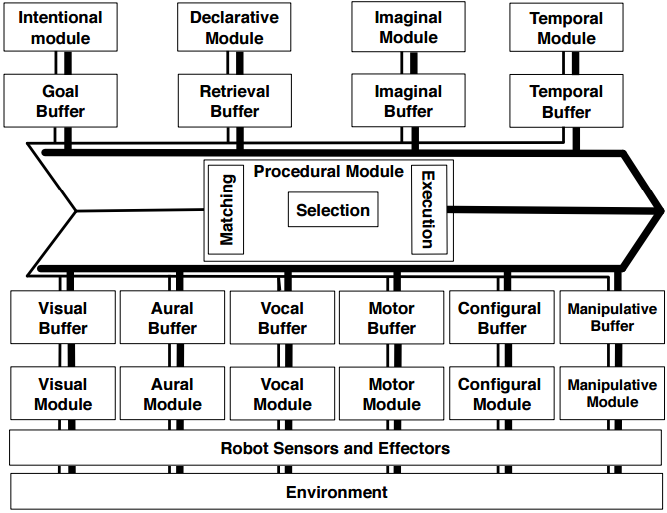
\includegraphics[width=0.8\textwidth]{actre}}
	\caption{ACT-R/E modules }
	\label{fig:modules}
\end{figure}

Most modules are identical to those of ACT-R. These include Intentional, Declarative, Imaginal, Speech, and Temporal modules with corresponding buffers. The detailed overview of ACT-R is presented in \cite{cosmos}, A.1.3\footnote{The architecture is named Adaptive Control of Thought - Rational in \cite{cosmos}.}

The data exchange is performed in \emph{chunks} of knowledge, a symbolic and sometimes subsymbolic information that can be placed in buffers.

The deciding module of both architectures is the procedural module. This module contains procedural knowledge and is able to choose a rule to fire basing on various information provided by other modules via their \emph{buffers}. 

A result of a production firing is an action performed by manipulators controlled with a motor module or a speech generated by the speech module. Additionally productions can instruct the agent to update its knowledge.

Other modules contain and maintain information such as declarative knowledge (declarative module), goal-oriented information (intentional module), time information (temporal module), and perceptive information (visual, aural modules). This information is appended with embodiment-related information in case of ACT-R/E. Embodiment-related information includes spatial perception information, manipulative information and movement information.

Spatial perception information contain information about ego-placement in the surroundings. It is handled by the configural buffer and made accessible to the procedural module via the configural buffer.

Manipulative information describes immediately graspable objects in an egocentric representation. It is maintained by the manipulative module and accessible via the manipulative buffer.

Movement information is presented by the motor module and may influence the current position in the configural module and objects in the manipulative module. 

Information from perceptive systems (i.e. what a robot sees) integrated with information from action modules (the motor module, i.e. what did a robot do) is encoded symbolically and subsymbolically and stored in the declarative module. This is a significant difference from the ACT-R architecture as the latter does not support movement and perceptual information encoded together as knowledge chunks with activation, thus a spreading activation basing on such information is impossible. In case of ACT-R/E perceptual and movement data are augmented and thus form a new knowledge chunk which, once accessed, can cause a spreading activation of relevant chunks.


\section {Characteristics}

The ACT-R/E architecture can be characterized according to the following table.

\begin{tabular}{|c|c|p{300pt}|}
\hline
Property & Value & Reason \\
\hline
Embodiment & + & Accounts for body location, manipulators, series of actions. Does not account for body properties affecting cognition (like chemical state), specific bodily properties of perception (like visual defects).\\
\hline
Perception & + & Same as ACT-R, plus perceptual-motor data augmentation. No in-detail description of how low-level perception is performed.\\
\hline
Action & + & Same as ACT-R. The motor and speech modules are actors of the agent. No details about the actions decomposition is given.\\
\hline
Anticipation & + & Same as ACT-R. Subsymbolic information and spreading activation help to anticipate, but no true internal modeling is performed. \\
\hline
Adaptation & + & Same as ACT-R plus the relation between perceptual and motion information. No development.\\ 
\hline
Motivation & & Same as ACT-R. Intentional module maintains goals as well as the current state within a goal. No means of internal goal deducing are proposed.\\
\hline
Autonomy & & Same as ACT-R, plus breaking the screen-as-a-world concept. No autonomous goals and development, no self-preservance, but addresses internal state maintaining.\\
\hline

\end{tabular}

\subsection{Additional characteristics}

The presented overview highlights a few additional characteristics that can be used to compare cognitive systems. We identify three such characteristics: timing, errors and optimality.

An architecture accounts for \emph{timing} if time is explicitly included in the architecture, affecting some or all processes within. ACT-R/E does account for timing strongly as it includes temporal measures of all processes. These measures strongly affect computation results.

\emph{Errors} are handled in an architecture if it models cognitive errors. ACT-R/E attempts to model errors of a human by managing subsymbolic information, including noise and modulating all computations with time.

\emph{Optimality} is concerned by an architecture design if an analysis of the speed, body requirements and computational hardware requirements (if any) is performed. Optimization of an architecture to increase speed or to lift the requirements improves the optimality coverage. ACT-R/E does not concern optimality, as explicitly stated in \cite{actre}. 

\section{Uncovered Concepts}

The article \cite{actre} covers the following concepts not covered in the Artificial Cognitive Systems course yet:

\begin{itemize}
	\item Analysis of models of a cognitive architecture.
	\item The task of modeling human cognition by a robot (cognition for cognition).
	\item Stochastic components of architectures used to model errors and noise.
	\item{[Mostly covered] Different types of memory.}
%	\item Spatial perception.
\end{itemize}

\begin{thebibliography}{2}
\bibitem{actre}{
	J. G. Trafton, L. M. Hiatt, A. M. Harrison, F. P. Tamborello, S. S. Khemlani, and A. C. Schultz. ACT-R/E: An embodied cognitive architecture for human-robot interaction. \emph{Journal of Human-Robot Interaction, 2(1): 30-55, 2013.}
}
\bibitem{actr1}{
	Anderson J.R. Act: A simple theory of complex cognition. 
	\emph{American Psychologist 51, pp. 355-365, 1996.}
}
\bibitem{actr2}{
	Anderson J.R., Bothell D. Byrne M.D., Douglass S., Lebiere C., Qin, Y. An integrated theory of the mind. 
	\emph{Psychological Review 111(4), pp. 1036-1060, 2004.}
}
\bibitem{cosmos}{
	D. Vernon, C. von Hofsten, and L. Fadiga. A Roadmap for Cognitive Development in Humanoid Robots 
	\emph{Cognitive Systems Monographs (COSMOS), Vol. 11, Springer,  2010.}
}
\end{thebibliography}

\end{document}